\documentclass[a4paper,12pt,twoside]{article}
\usepackage[a4paper,top=25mm,bottom=25mm,left=35mm,right=25mm]{geometry}
\usepackage{blindtext}
\usepackage[utf8]{inputenc}
\usepackage{graphicx}
\usepackage[export]{adjustbox}
\usepackage{ifpdf}
\usepackage[table]{xcolor}
\usepackage{amsmath,amsthm}
\usepackage{listings}
\usepackage{graphicx}
\usepackage{epsfig, rotating, latexsym, amssymb, pstricks}
\usepackage[numbers]{natbib}
\usepackage{setspace} 
\usepackage{array}
\usepackage{overpic}
% define column for aligning numbers in tables
\usepackage{dcolumn}
\newcolumntype{d}[1]{D{.}{.}{#1}}
\usepackage{wrapfig}

\usepackage[caption=false,font=footnotesize]{subfig}
% \usepackage{natbib}
\usepackage[slovene,english]{babel}
%\usepackage[bookmarks, colorlinks=true, plainpages=false, 
%            citecolor=blue, linkcolor=blue, filecolor=blue]{hyperref}
\usepackage[bookmarks, colorlinks=true, plainpages=false,
            citecolor=black, linkcolor=black, filecolor=black,
            breaklinks=true]{hyperref}
\usepackage{bashful}
% do not reset footnote numbers for each chapter
\usepackage{chngcntr}

\usepackage[none]{hyphenat} %to prevent word splitting
\setlength{\parindent}{0em}
\setlength\bibsep{6pt}

\newenvironment{scriptdata}%
  {\vspace{3mm}\begin{list}{$\bullet$}{%
        \renewcommand{\makelabel}[1]{\textbf{##1}\hfil}%
        \setlength{\labelwidth}{17mm}%
        \setlength{\labelsep}{1mm}%
        \setlength{\leftmargin}{18mm}%
        \setlength{\itemsep}{0mm}%
        \setlength{\topsep}{0mm}%
        \setlength{\partopsep}{0mm}%
        \setlength{\parskip}{0mm}%
        \setlength{\parsep}{0mm}}}
  {\end{list}\vspace{3mm}}
  

\begin{document}

\pagestyle{plain}
\addtolength{\baselineskip}{0.4ex} % Dodatni razmik med vrsticami

% Define pagestyle
\renewcommand{\sectionmark}[1]{\markright{\thesection\ \ #1}}

% from now on, add extra line between paragraphs
\addtolength{\parskip}{\baselineskip}
%\doublespacing


\title{ParaView ReadUALEdge plugin\\tutorial}
\author{Dejan Penko\\
University of Ljubljana}
\date{August 2016}

\maketitle

%\section{Introduction}

%\clearpage
\graphicspath{ {images/} }
\singlespacing
\tableofcontents
\clearpage

\section{\textbf{Introduction}}

This paper will cover the basic instructions about running and using ParaView application\footnote[1]{During the time of writing this paper ParaView version 5.1.0 was used} and how to run and use ReadUALEdge ParaView plugin on g04.efda-itm.

\section{\textbf{ParaView}}

ParaView is an open-source, multi-platform application used to visualize data sets. Here we won't cover the installation process as the all needed informations including setup guide, tutorials etc. can be found on ParaView wiki page \\ \textit{http://www.paraview.org/Wiki/ParaView} and in ParaView Guide found on \\ \textit{http://www.paraview.org/paraview-guide/}.

The use of some useful ParaView tools will be covered in ReadUALEdge plugin chapter.


\section{\textbf{ParaView ReadUALEdge plugin}}

ParaView ReadUALEdge plugin is a tool used to visualize and analyze data, obtained by fusion simulations (electron temperature/density, ion temperature/density) stored in CPO and/or IDS database. 

Here we'll demonstrate how to launch and use the ReadUALEdge plugin using two different IDS databases, first being shot: 16151; run: 1000 \footnote[2]{user: kosl; tokamak: aug; version: 4.10a.} and  shot: 1; run: 1 \footnote[3]{user: kosl; tokamak: aug; version: 4.10a. IDS database for now doesn't take in those three parameters as the CPO database does.}

Note that because we are using IDS database, the following modules must be loaded using terminal commands:

\begin{itemize}
\item[] \%module use -a ~dkaljun/imas/etc/modulefiles
\item[] \%module load imas/develop/3/ual/develop\\ \\
Additional commands to check available modules etc.:
\item[] \%module avail imas
\item[] \%module display imas/develop/3/ual/develop
\end{itemize}

\clearpage
\subsection{Loading the plugin}

After launching the ParaView application the start window appears. The main parts, as seen in Fig. \ref{fig:pv_start_window} are: 

\begin{itemize}
\item[1.] Menu bar
\item[2.] Toolbar
\item[3.] Pipeline Browser
\item[4.] View Browser
\end{itemize}

\begin{figure}[ht] \centering
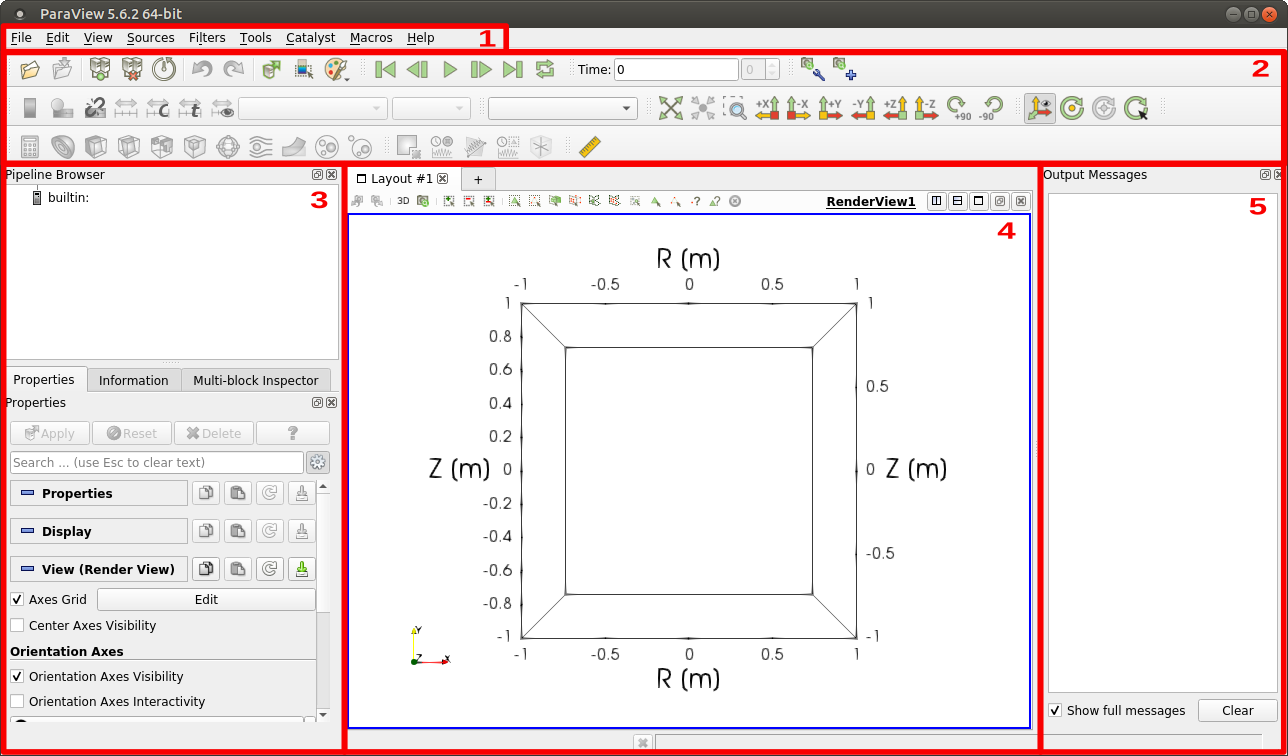
\includegraphics[scale=0.5,trim=0cm 0cm 0cm 0cm,clip]{1_start_window_marked}
	\caption{ParaView start window}
	\label{fig:pv_start_window}
\end{figure}


\clearpage
Loading and running the ReadUALEdge plugin is done in the next few steps:

\begin{itemize}
    \item[1.]{Open the \textbf{Plugin Manager} by navigating from Menu Bar to \textit{Tools} $\to$ \textit{Manage Plugins} (see Fig. \ref{fig:pv_manage_plugins})}
    \begin{figure}[ht] \centering
        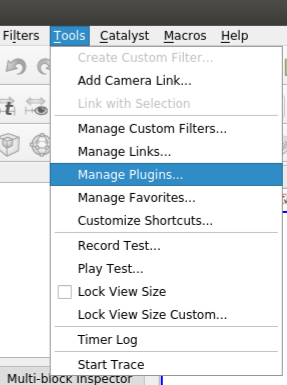
\includegraphics[scale=0.5,trim=0cm 0cm 0cm 0cm,clip]{2_manage_plugins}
    	\caption{Navigating to the Plugin Manager}
    	\label{fig:pv_manage_plugins}
    \end{figure}

    \item[2.]{In Plugin Manager press the \textbf{Load Now} button (see Fig. \ref{fig:pv_plugin_manager_1})}
    \begin{figure}[ht] \centering
    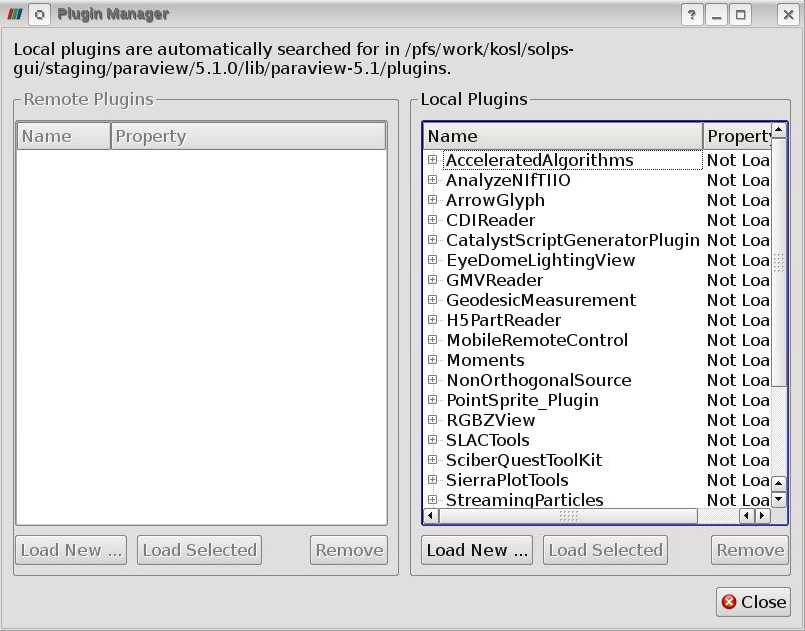
\includegraphics[scale=0.5,trim=0cm 0cm 0cm 0cm,clip]{3_plugin_manager1}
    	\caption{Plugin Manager window}
    	\label{fig:pv_plugin_manager_1}
    \end{figure}
    \clearpage
    \item[3.]{Navigate to and select the plugin library file then press \textbf{OK} (see Fig. \ref{fig:pv_plugin_manager_2})}
    \begin{figure}[ht] \centering
        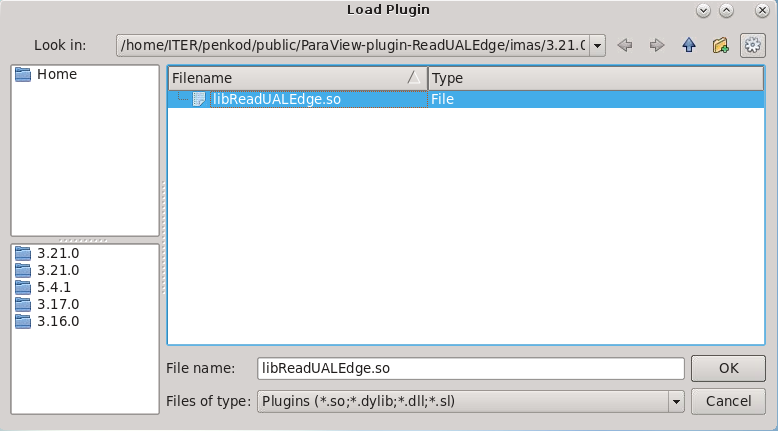
\includegraphics[scale=0.5,trim=0cm 0cm 0cm 0cm,clip]{4_plugin_manager2}
    	\caption{Navigating and selecting plugin library file}
    	\label{fig:pv_plugin_manager_2}
    \end{figure}
    
    \item[4.]{Now the plugin should be already loaded. If it's not, highlight the plugins name in Plugin Manager and press \textbf{Load Selected} button. Optionally by checking the \textbf{Auto Load} option the plugin will be automatically loaded whenever the ParaView application is launched (see Fig. \ref{fig:pv_plugin_manager_3})}
    \begin{figure}[ht] \centering
        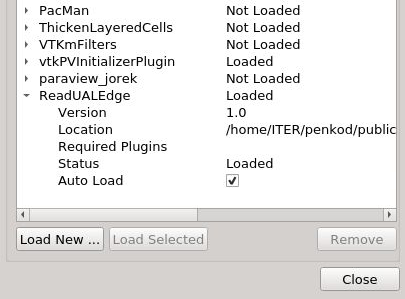
\includegraphics[scale=0.5,trim=0cm 0cm 0cm 0cm,clip]{5_plugin_manager3}
    	\caption{Loading the ReadUALEdge plugin}
    	\label{fig:pv_plugin_manager_3}
    \end{figure}
    \clearpage
    
    \item[5.]{Run the plugin by navigating from Menu Bar to \textit{Sources} $\to$ \textit{UAL Edge} (see Fig. \ref{fig:pv_run_plugin_1}). The Pipeline Browser will change and after choosing the desired database parameters press button \textbf{Apply} (see Fig. \ref{fig:pv_run_plugin_2}). The database will be loaded and visualized on the View Browser as seen in Fig. \ref{fig:pv_run_plugin_3} for Aug tokamak and in Fig. \ref{fig:pv_run_plugin_4} for Iter tokamak.}
    \vspace{2cm}
    \begin{figure}[ht] \centering
        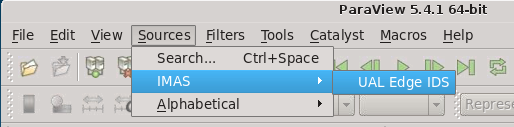
\includegraphics[scale=0.5,trim=0cm 0cm 0cm 0cm,clip]{6_running_plugin}
    	\caption{Running the ReadUALEdge plugin}
    	\label{fig:pv_run_plugin_1}
    \end{figure}
    
    \begin{figure}[ht] \centering
        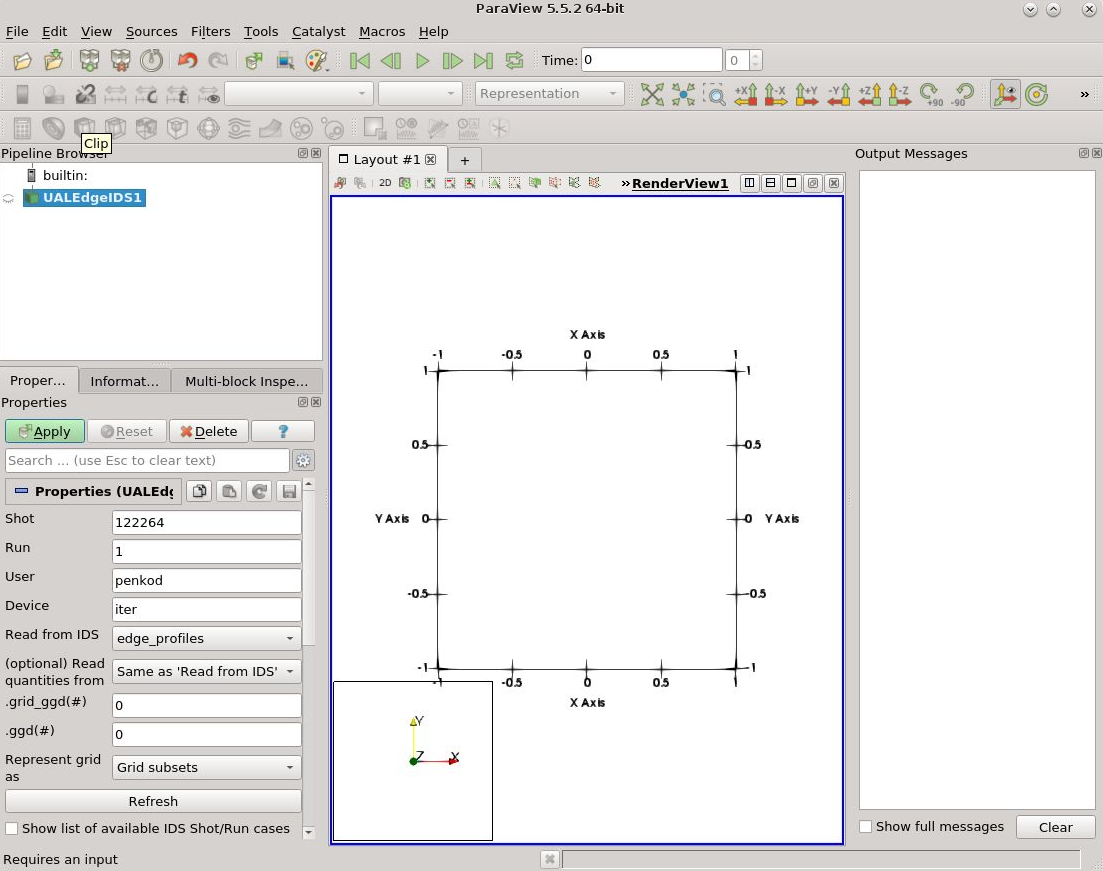
\includegraphics[scale=0.5,trim=0cm 0cm 0cm 0cm,clip]{7_plugin_run1}
    	\caption{Applying the ReadUALEdge plugin database parameters}
    	\label{fig:pv_run_plugin_2}
    \end{figure}
    
    \begin{figure}[ht] \centering
        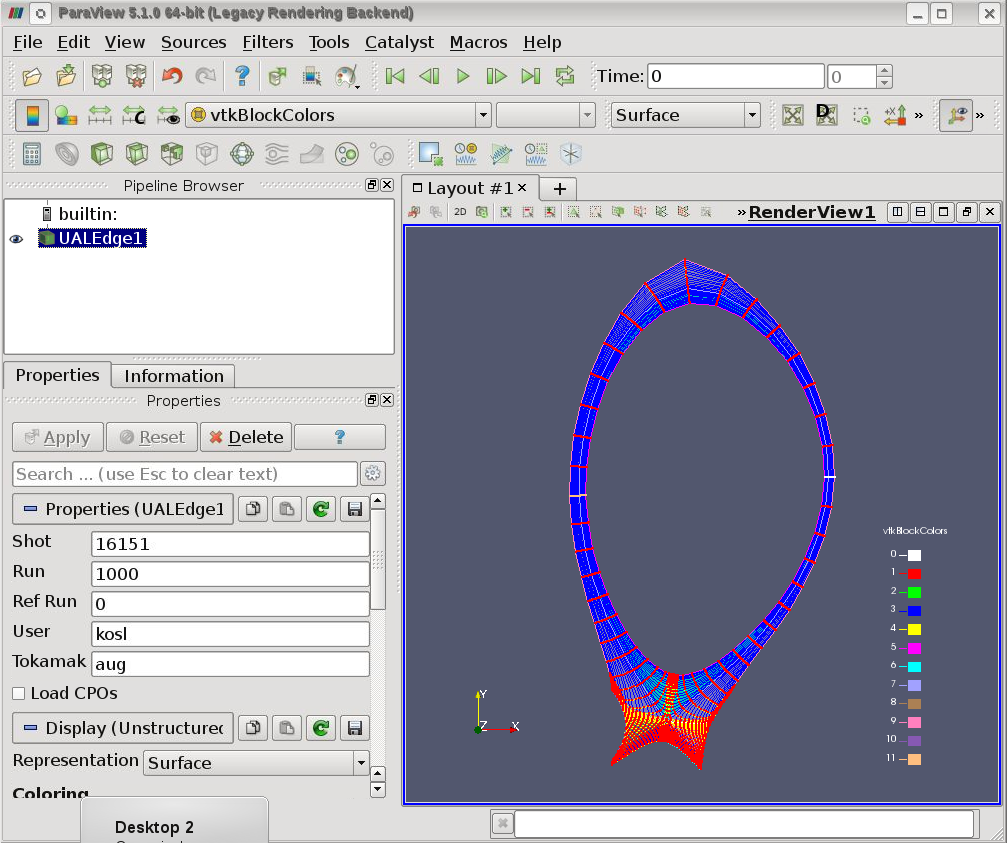
\includegraphics[scale=0.5,trim=0cm 0cm 0cm 0cm,clip]{8_plugin_run2}
    	\caption{Example of visualized data gathered from tokamak $Aug$ database}
    	\label{fig:pv_run_plugin_3}
    \end{figure}
    \clearpage
    
    \begin{figure}[ht] \centering
        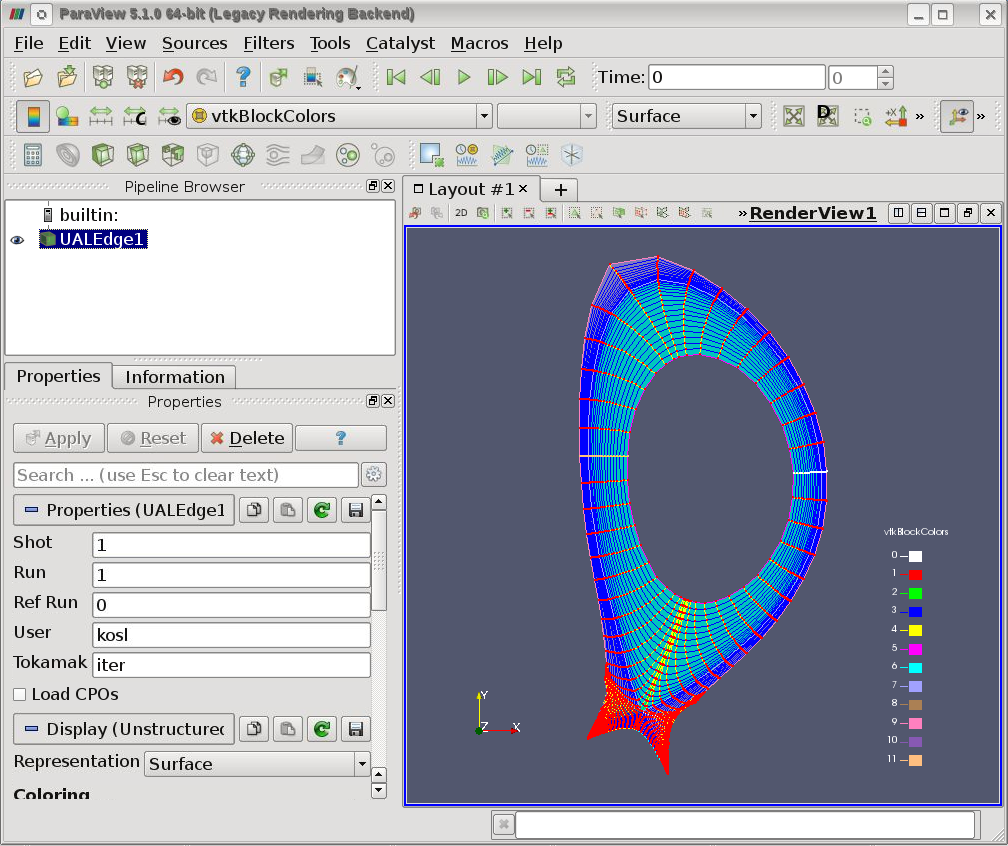
\includegraphics[scale=0.5,trim=0cm 0cm 0cm 0cm,clip]{10_plugin_loaded3}
    	\caption{Example of visualizied data gathered from tokamak $Iter$ database}
    	\label{fig:pv_run_plugin_4}
    \end{figure}
\end{itemize}

\begin{wrapfigure}{r}{0.35\textwidth}
\hspace{1.5cm}
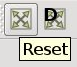
\includegraphics[scale=1,trim=0cm 0cm 0cm 0cm,clip]{9_reset_button}
	\caption{Reset button}
	\label{fig:pv_reset_button}
\end{wrapfigure}

Note: Sometimes after opening Iter tokamak database \textbf{no} visual change in the $View$ $Browser$ can be seen, because of the default zoom. To solve that press twice the \textbf{Reset button} found in \textit{Toolbar}

\clearpage
\subsection{Data analysis}

In previous chapter we can notice that we have loaded data, but no useful information could be seen, just the geometry of the tokamak using a lot of colors. In this chapter we'll first explain what those multiple color represent and then how to display full information we want.

\subsubsection{Subgrids and Multi-Block Inspector}

Briefly said, subgrid is "a piece" of geometry\footnote[1]{More information about subgrids can be found in \textit{Edge cpo2ids converter work notes} .pdf}. In our case, the \textbf{Multi-Block Inspector} uses the subgrids as blocks of data, using a different color for each block of data, as seen in Figures \ref{fig:pv_run_plugin_3} and \ref{fig:pv_run_plugin_4}, and it is used to select and display only the wanted blocks of data.

To load the Multi-Block Inspector, go to Menu bar $View$ and check the \textit{Multi-Block Inspector} selection, as seen in Fig. \ref{fig:pv_loading_mbinsp}. Then you should have already noticed that a new interface called \textit{Multi-Block Inspector} opened at the bottom of the Pipeline Browser, as seen in Fig. \ref{fig:pv_mbinsp}.

\begin{figure}[ht] \centering
\begin{minipage}[b]{0.5\textwidth}
    \centering
    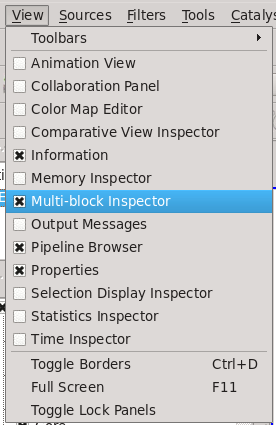
\includegraphics[scale=0.5,trim=0cm 0cm 0cm 0cm,clip]{11_loading_mbinsp}
    \vspace{1cm}
    \caption{Loading the Multi-Block Inspector}
    \label{fig:pv_loading_mbinsp}
\end{minipage}%
\begin{minipage}[b]{0.5\textwidth}
    \centering
    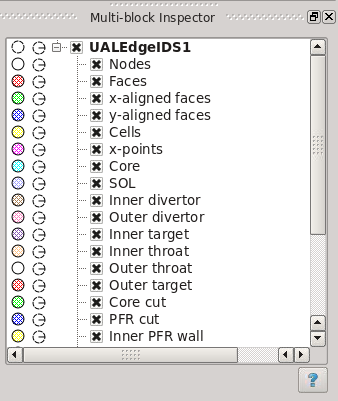
\includegraphics[scale=0.5,trim=0cm 0cm 0cm 0cm,clip]{12_mbinsp}
    \caption{Multi-Block Inspector}
    \label{fig:pv_mbinsp}
\end{minipage}
\end{figure}

\clearpage

Here we can select the wanted blocks we want to be seen in the \textit{View Browser}. An example is shown in Fig. \ref{fig:pv_mbinscp_cells}, where only the $Cells$ block was selected, and in Fig. \ref{fig:pv_mbinscp_nodes}, where only the $Nodes$ block was selected. We can also choose multiple blocks at once, as shown in Fig. \ref{fig:pv_mbinspc_sol_odivertor} where blocks $SOL$ and $Outer$ $Divertor$ were selected.

\begin{figure}[ht] \centering
    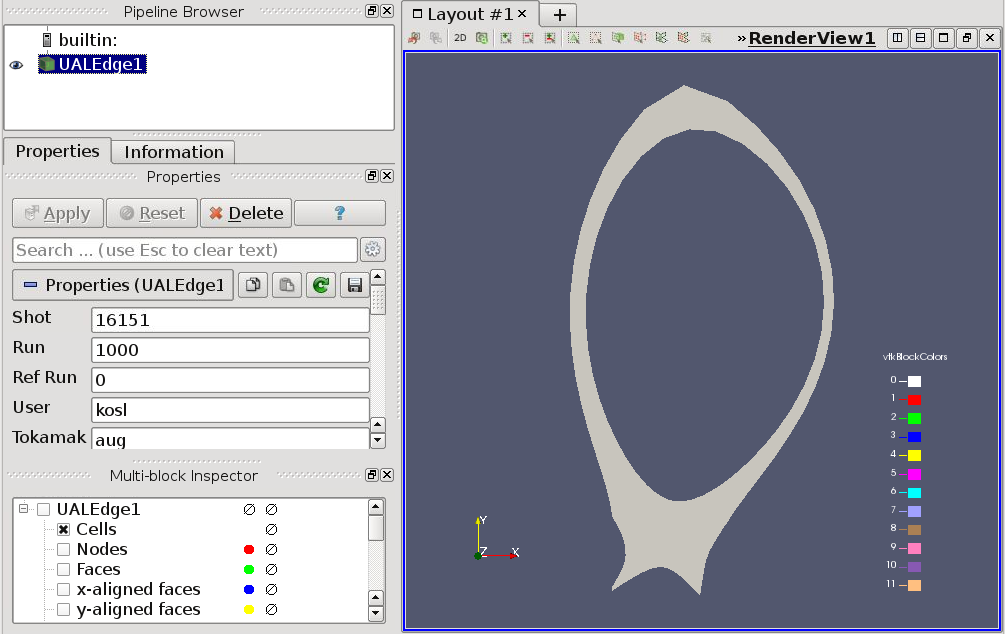
\includegraphics[scale=0.5,trim=0cm 0cm 0cm 0cm,clip]{13_mbinsp_cells}
    \caption{Displaying Cells block using Multi-Block Inspector}
    \label{fig:pv_mbinscp_cells}
\end{figure}

\vspace{1cm}

\begin{figure}[!htb] \centering
    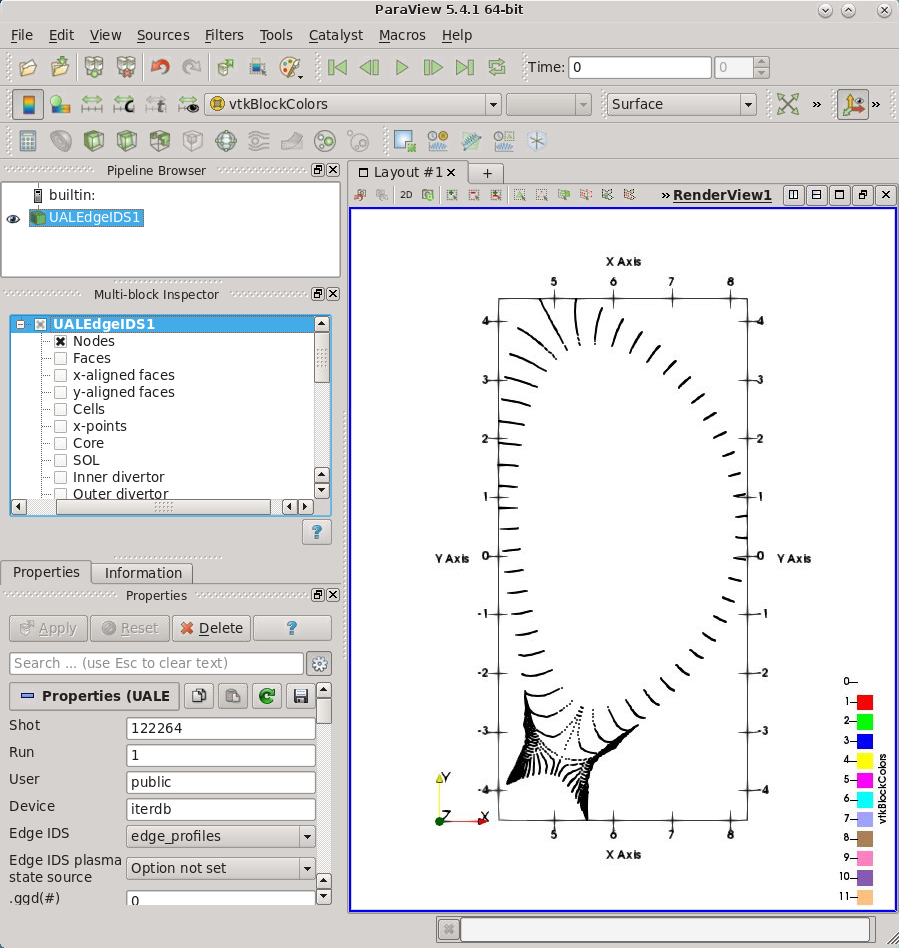
\includegraphics[scale=0.5,trim=0cm 0cm 0cm 0cm,clip]{14_mbinsp_nodes}
    \caption{Displaying Nodes block using Multi-Block Inspector}
    \label{fig:pv_mbinscp_nodes}
\end{figure}
\clearpage
\begin{figure}[!htb] \centering
    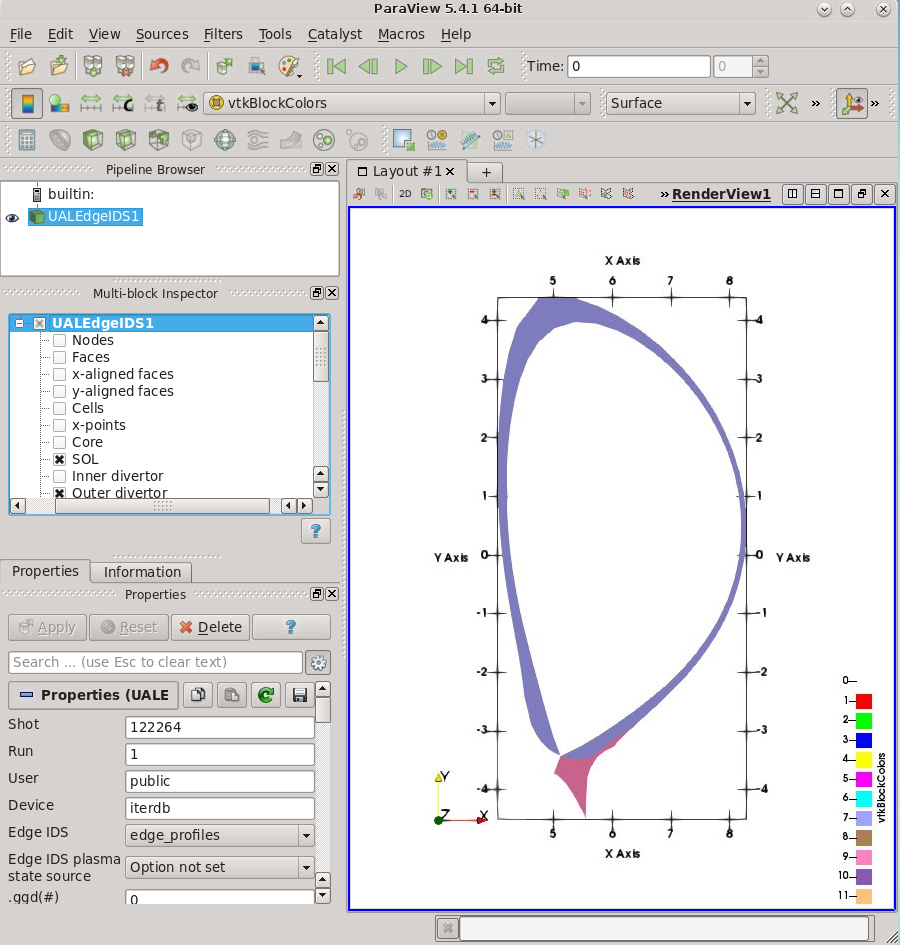
\includegraphics[scale=0.5,trim=0cm 0cm 0cm 0cm,clip]{15_mbinsp_sol-odivertor}
    \caption{Displaying SOL and Outer Divertor blocks using Multi-Block Inspector}
    \label{fig:pv_mbinspc_sol_odivertor}
\end{figure}

\clearpage 
\subsubsection{Data arrays}

Data arrays are holding data such as \textit{electron density/temperature} and \textit{ion density/temperature} values, which are used to color the blocks. When running the ReadUALedge plugin with the \textit{Multi-Block Inspector} the \textit{vtkBlockColors} layer is automatically selected, coloring the blocks with their specific block color. To select the wanted data layer navigate through \textbf{List of Data Arrays} found in Toolbar, as seen in Fig. \ref{fig:pv_data_arrays_list}. Examples are shown in Figures \ref{fig:pv_data_arrays_list_ne}, \ref{fig:pv_data_arrays_list_te} and \ref{fig:pv_data_arrays_list_te_core_sol}.

\begin{figure}[ht] \centering
    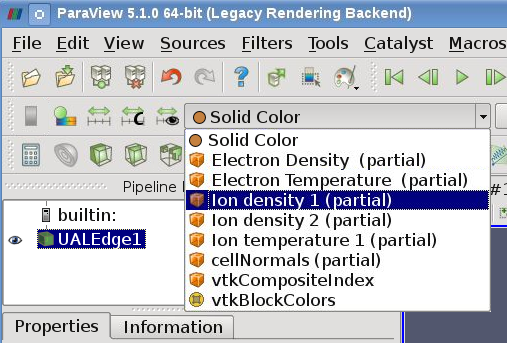
\includegraphics[scale=0.5,trim=0cm 0cm 0cm 0cm,clip]{16_data_arrays_list}
    \caption{List of data arrays}
    \label{fig:pv_data_arrays_list}
\end{figure}

\begin{figure}[ht] \centering
    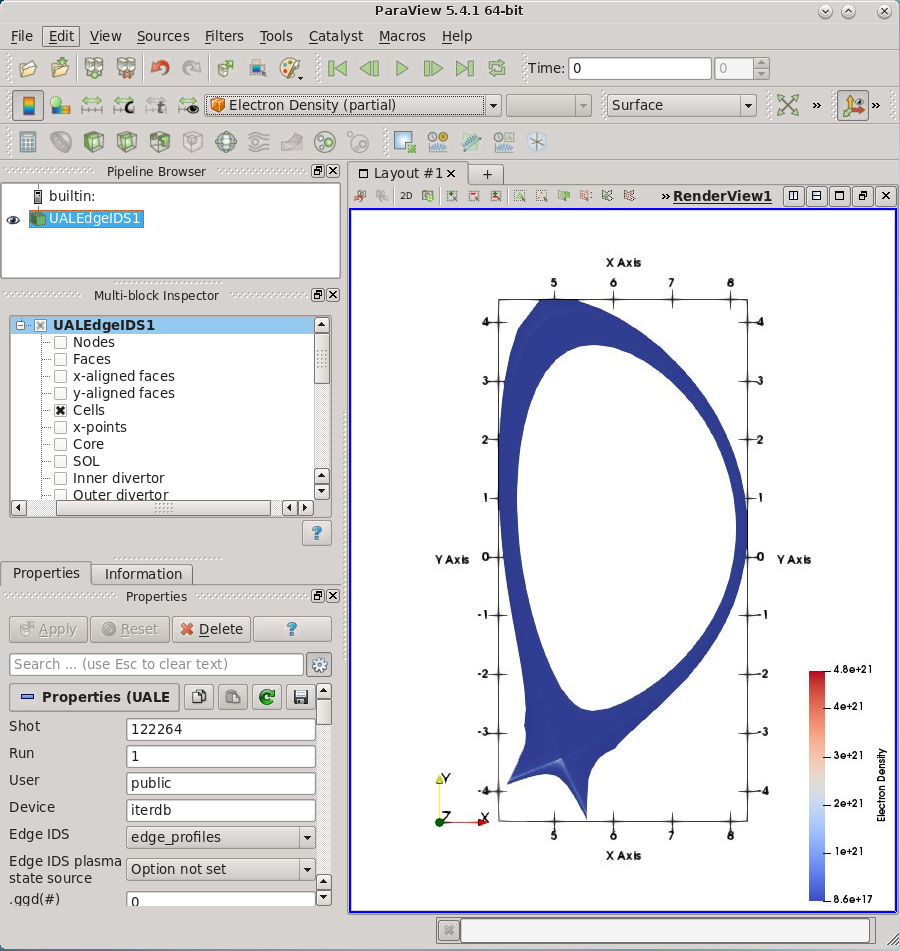
\includegraphics[scale=0.5,trim=0cm 0cm 0cm 0cm,clip]{17_data_arrays_ne_full}
    \caption{Data layer Electron Density using Cell block}
    \label{fig:pv_data_arrays_list_ne}
\end{figure}

\begin{figure}[ht] \centering
    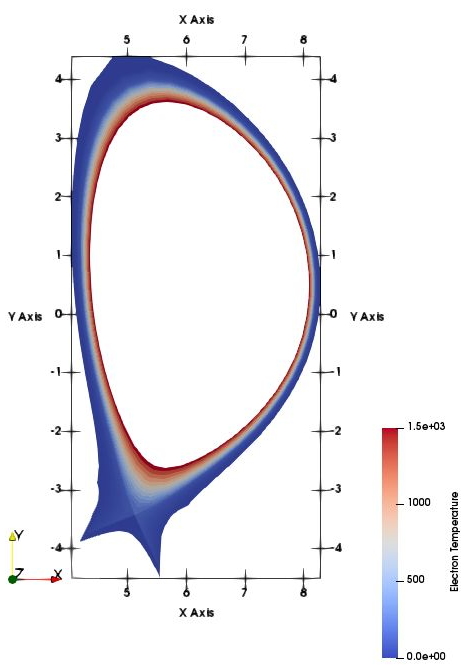
\includegraphics[scale=0.5,trim=0cm 0cm 0cm 0cm,clip]{18_data_arrays_te}
    \caption{Data layer Electron Temperature using Cell block}
    \label{fig:pv_data_arrays_list_te}
\end{figure}

\begin{figure}[ht] \centering
    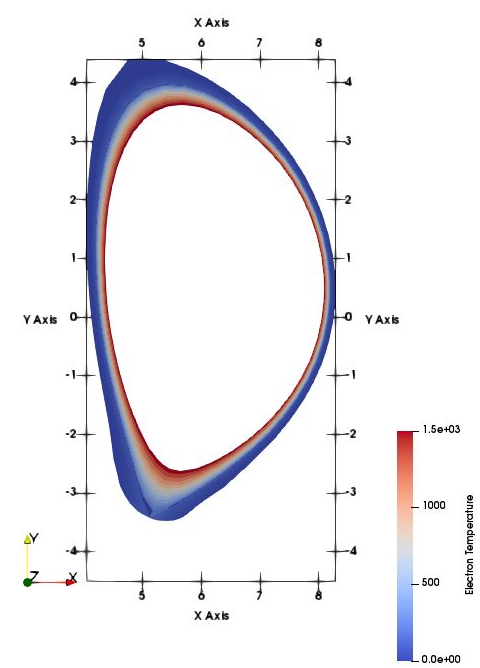
\includegraphics[scale=0.5,trim=0cm 0cm 0cm 0cm,clip]{19_data_arrays_te_core_sol}
    \caption{Data layer Electron Temperature using Core and SOL block}
    \label{fig:pv_data_arrays_list_te_core_sol}
\end{figure}

\clearpage

\subsection{Other useful ParaView tools}

\subsubsection{Python Calculator filter}

Python Calculator filter allows us to work with data arrays (Electron Density, Ion Temperature etc.) and create new data array to display the results. It can be found under $Filter\to Alphabetical\to Python$ $Calculator$ as seen in Fig. \ref{fig:pv_python_calculator1} and \ref{fig:pv_python_calculator2}.

\begin{figure}[ht] \centering
\begin{minipage}[b]{0.48\textwidth}
    \centering
    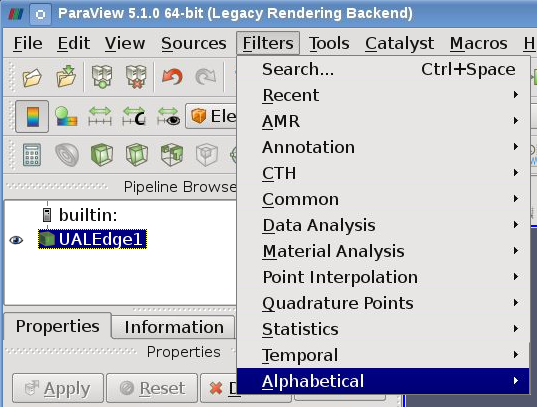
\includegraphics[scale=0.5,trim=0cm 0cm 0cm 0cm,clip]{20_python_calculator1}
    \caption{}
    \label{fig:pv_python_calculator1}
\end{minipage}\hfill
\begin{minipage}[b]{0.48\textwidth}
    \centering
    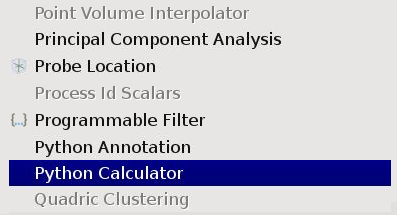
\includegraphics[scale=0.5,trim=0cm 0cm 0cm 0cm,clip]{21_python_calculator2}
    \vspace{1.5cm}
    \caption{}
    \label{fig:pv_python_calculator2}
\end{minipage}
\end{figure}

After selecting the Python Calculator a new interface will open in the Pipeline Browser as seen in Fig. \ref{fig:pv_python_calculator3}. 

\begin{figure}[ht] \centering
    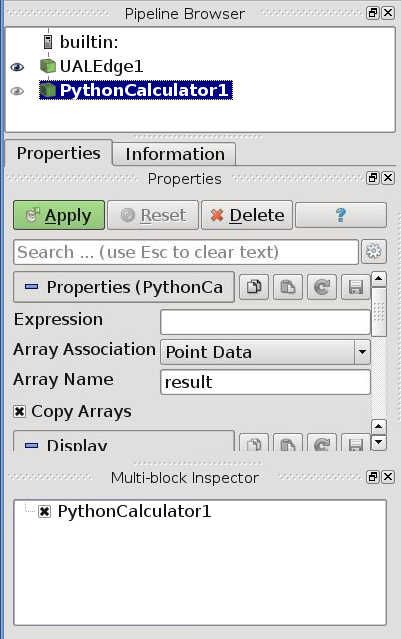
\includegraphics[scale=0.5,trim=0cm 0cm 0cm 0cm,clip]{22_python_calculator3}
    \caption{Python Calculator start in Pipeline Browser}
    \label{fig:pv_python_calculator3}
\end{figure}

\clearpage 

This filter takes a case sensitive \textit{Expression}\footnote[1]{The Python Calculator \textbf{does not} take in Python code expression/syntax! It takes in already defined functions and their parameters.}, an \textit{Array Association} and custom \textit{Array Name}. An example is shown in Fig. \ref{fig:pv_python_calculator4}, where we used next expression and options:

\begin{itemize}
\item  Expression: \\ inputs[0].CellData['Ion Density 1']+inputs[0].CellData['Ion Density 2']
\item  Array Association: \\ Cell Data
\item  Array Name: \\ Custom Array Name
\item   Press Apply Button
\end{itemize}

\begin{figure}[ht] \centering
    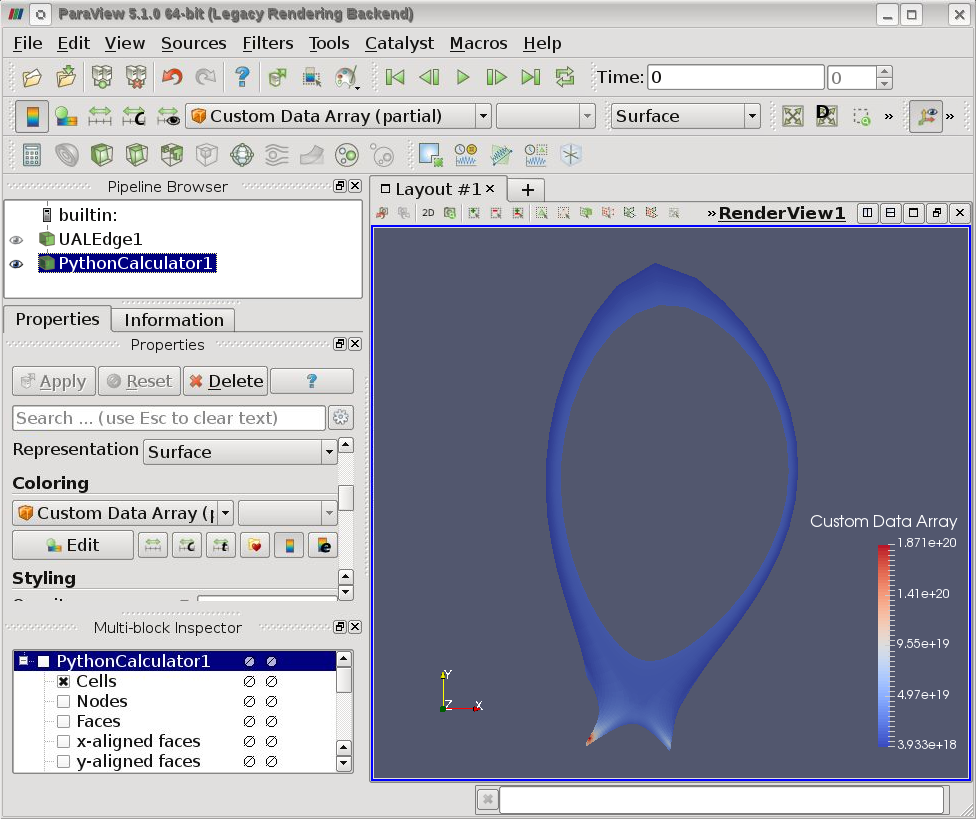
\includegraphics[scale=0.5,trim=0cm 0cm 0cm 0cm,clip]{23_python_calculator4}
    \caption{Sum of Ion Density arrays scalars as Custom Data Array}
    \label{fig:pv_python_calculator4}
\end{figure}

In this case the Python Calculator created a sum of \textit{Ion Density 1} and \textit{Ion Density 2} data arrays and created new data array called \textit{Custom Array Name}, which can be chosen from the Data Array list and analyzed.

\clearpage 

Note 1: If we have a long list od data layers and want to create sum of all of them the expression can be very long. Typing it manually can be frustrating, so it's advisable to use a short self written script to generate the expression. ParaView includes also its own Python Shell. The use of Python Shell in Paraview and example of script to generate the expression is explained and shown in \textit{ParaView Python Shell} chapter.

Note 2: After the Python Calculator was ran and until applying the setting in Pipeline Browser there will be one block shown in Multi-Block Inspector, if activated, with the name $PythonCalculator1$. If we deselect this block, the ParaView might crash and it may also cause the ReadUALEdge plugin to fully unload, in which case it must be again manually loaded using Plugin Manager. 
After pressing the \textbf{Apply} button the Multi-Block Inspector works normally. 

More Python Calculator functions and operations can be found on web page \\
$http://www.itk.org/Wiki/index.php?title=ParaView/Users\_Guide/ \\ Python\_Calculator\&oldid=46066$ \\
and in ParaView guide under Chapter 5.8.2.

\clearpage 
\subsubsection{ParaView Python Shell}

ParaView Python Shell\footnote[1]{uses Python 2.6.9} can be found navigating to $Tools \to Python Shell$ and it opens Paraview editor as shown in Fig. \ref{fig:pv_python_shell} and \ref{fig:pv_python_shell2}.

\begin{figure}[ht] \centering
    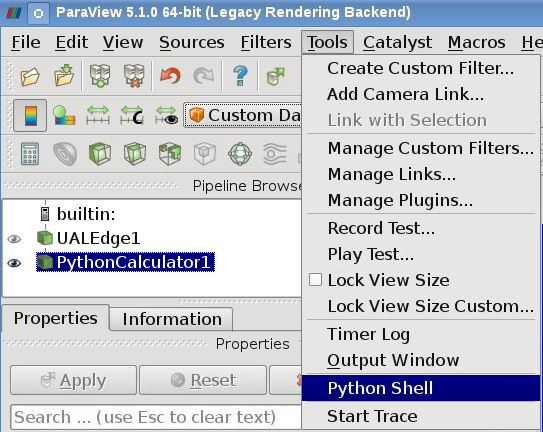
\includegraphics[scale=0.5,trim=0cm 0cm 0cm 0cm,clip]{24_python_shell}
    \caption{Navigating to ParaView Shell}
    \label{fig:pv_python_shell}
\end{figure}

\begin{figure}[ht] \centering
    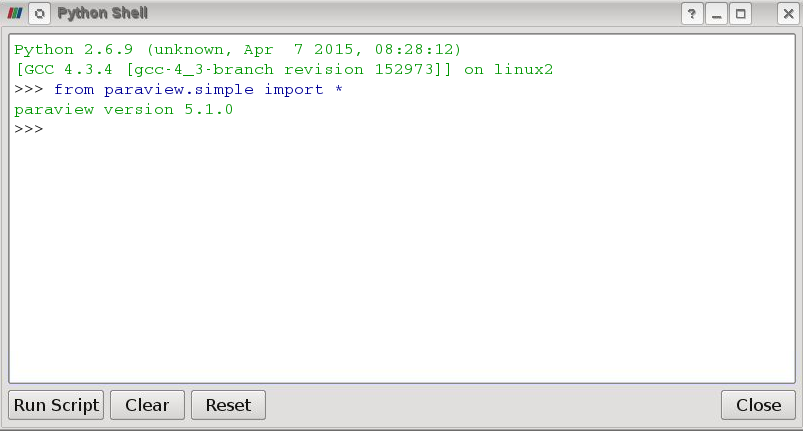
\includegraphics[scale=0.5,trim=0cm 0cm 0cm 0cm,clip]{25_python_shell2}
    \caption{ParaView Python Shell window}
    \label{fig:pv_python_shell2}
\end{figure}

Here we'll show an example solving the issue with quite long Python Calculator Expressions. 
The IDS database Shot:1; Run:1; User: kosl; Tokamak: Iter has almost 100 Ion Density data arrays, so very long expression is needed to create a sum of all of them, but because inside the expression the functions are being repeated we can easily generate it using Python Shell.

\clearpage

The Python script and part of its output is shown in Fig. \ref{fig:pv_python_shell3}.

\begin{figure}[ht] \centering
    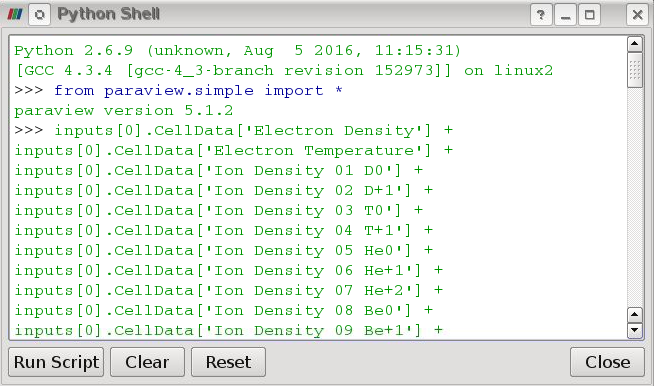
\includegraphics[scale=0.5,trim=0cm 0cm 0cm 0cm,clip]{26_python_shell3}
    \caption{Python Shell code and output}
    \label{fig:pv_python_shell3}
\end{figure}

The results of using the mentioned IDS database and the generated expression by copying it are shown in Fig. \ref{fig:pv_python_calculator5}.

\begin{figure}[!htb] \centering
    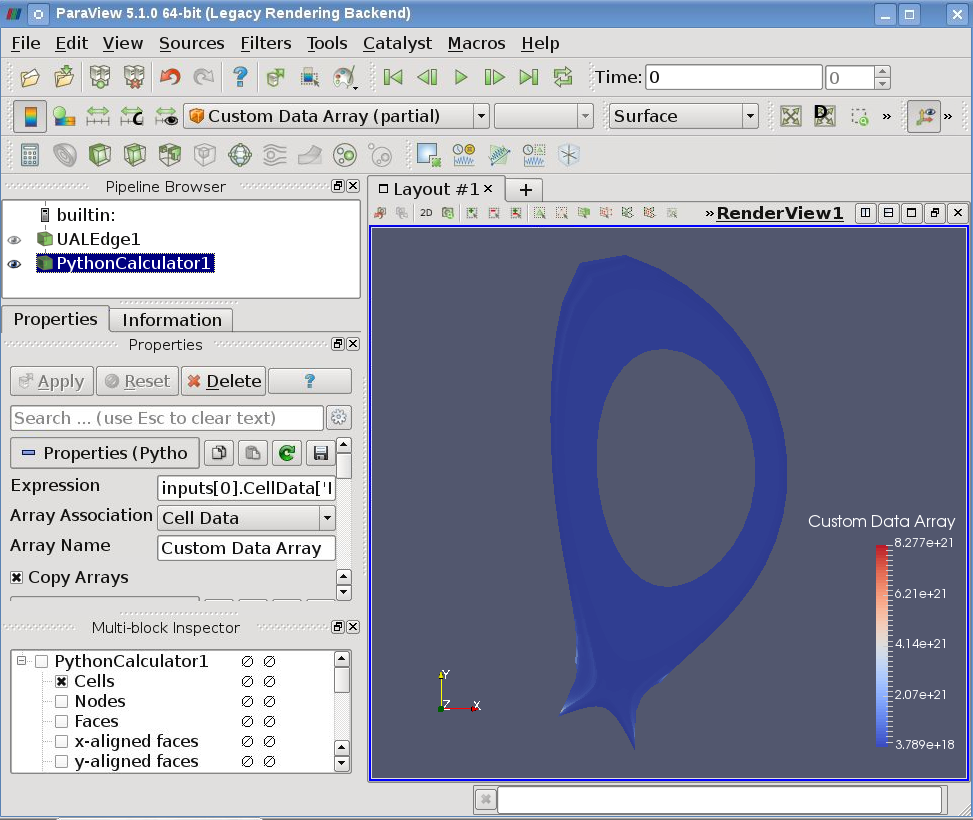
\includegraphics[scale=0.5,trim=0cm 0cm 0cm 0cm,clip]{27_python_calculator5}
    \caption{IDS Iter tokamak and Custom Data Array as sum of all Ion Density arrays scalars}
    \label{fig:pv_python_calculator5}
\end{figure}

\clearpage
\subsubsection{Plot Over Line filter}

Plot Over Line filter is a flexible tool, used to create a chart such as temperature change through the wall. 

The start and end location of the plotted data is user selected, and the plot values are taken from available Data Arrays and also from coordinates of previously mentioned start and end location.

It can be found at the same location as any other filter, navigating to $Filters \to Alphabetical \to Plot \ Over\ Line$, as seen in Fig. \ref{fig:pv_pov1}. When selected, two by line connected white dots, representing the start and end location taken for the plot, will appear on the \textit{View Browser}, as seen in Fig. \ref{fig:pv_pov2}, which can be moved by clicking and dragging with the mouse pointer. When done, press the \textbf{Apply} button. 

\begin{figure}[!htb] \centering
    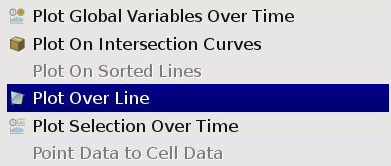
\includegraphics[scale=0.5,trim=0cm 0cm 0cm 0cm,clip]{28_pov1}
    \caption{Navigating to Plot Over Line filter}
    \label{fig:pv_pov1}
\end{figure}

\begin{figure}[!htb] \centering
    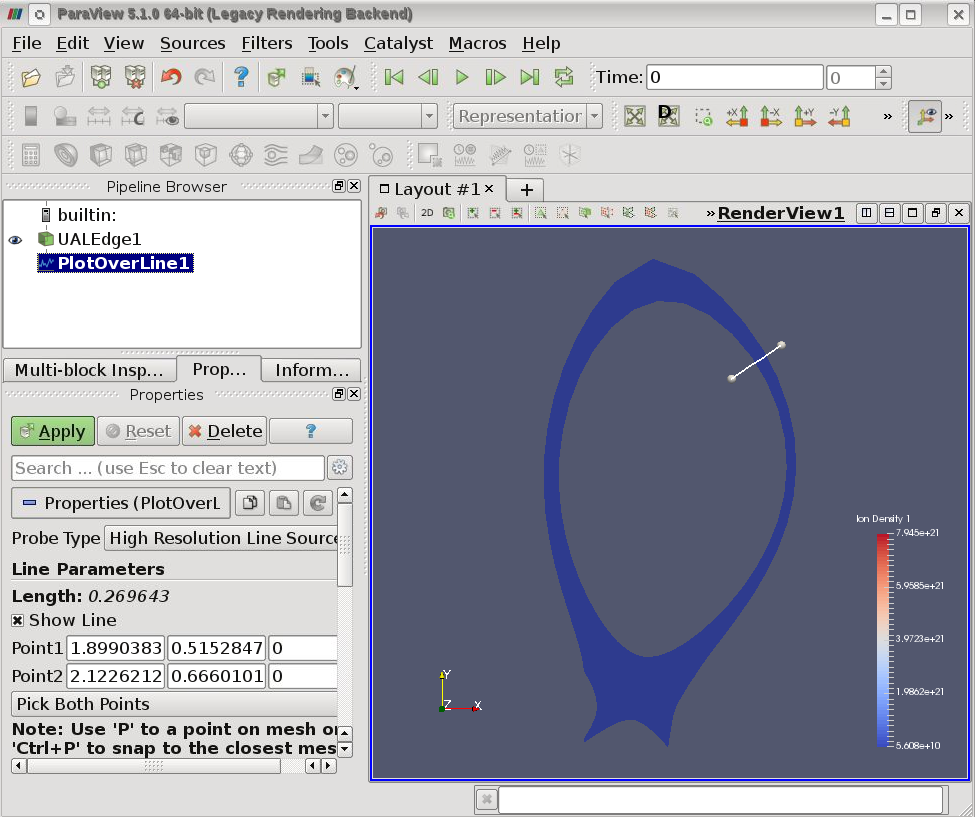
\includegraphics[scale=0.5,trim=0cm 0cm 0cm 0cm,clip]{29_pov2}
    \caption{Selecting end and start location for the plot}
    \label{fig:pv_pov2}
\end{figure}

\clearpage 

By pressing the \textbf{Apply} button a new interface will appear in the \textit{Pipeline Browser} and also the default chart will appear on the \textit{View Browser}, as seen in Fig. \ref{fig:pv_pov3}. 

\begin{figure}[!htb] \centering
    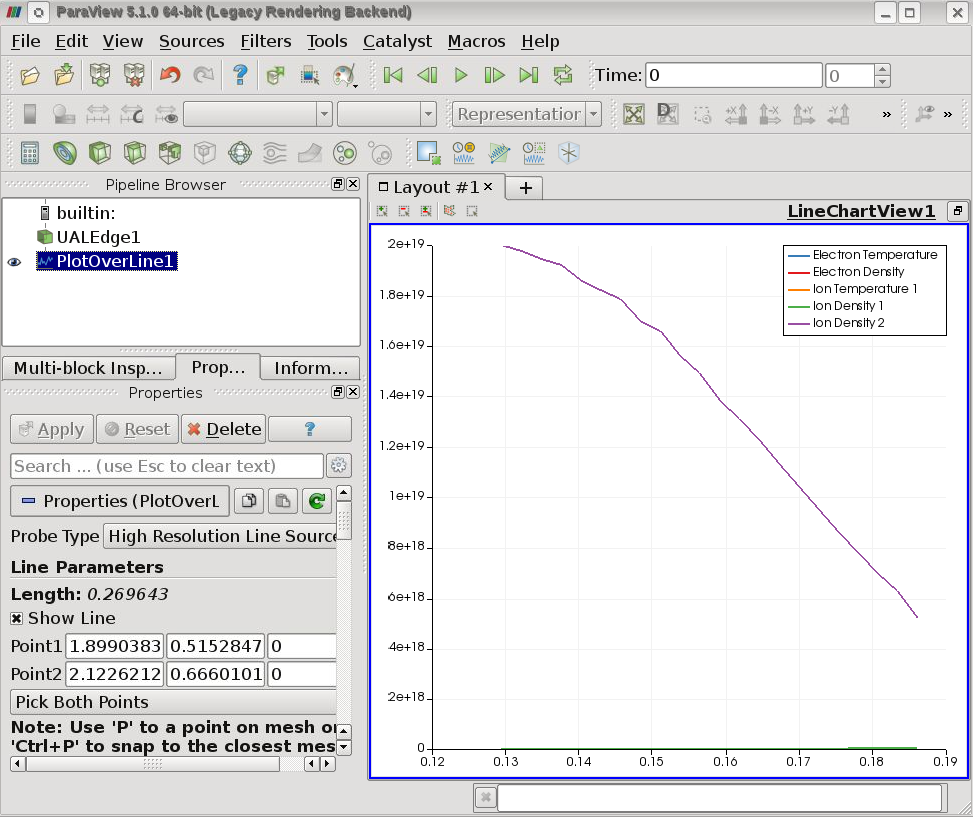
\includegraphics[scale=0.35,trim=0.05cm 0cm 0.15cm 0cm,clip]{30_pov3}
    \caption{Chart example}
    \label{fig:pv_pov3}
\end{figure}

You can notice, that all the Data Arrays are being shown in the chart and also making some of them unclear because of the used  value range. Note also that by default the X-axis is following the direction and length of the previously for the plot selected start and end point.

There are many different settings to get the desired chart view, here a few of them will be shown.

The simplest one is by clicking the left mouse button on the chart and by dragging the line by mouse.

\clearpage
To display only the selected Data Array data, in the new \textit{Pipeline Browser} interface scroll down to \textbf{Series Parameters} and there the desired Data Arrays (and also showing coordinate changes from start to end point) can be chosen, as seen in Fig. \ref{fig:pv_pov4}. The range will automatically adjust to selected plot values.

Chart line colors can be changed double clicking the colored square icon in the \textit{Series Parameters} and \textbf{Choose Series Color} window will appear.

\begin{figure}[!htb] \centering
    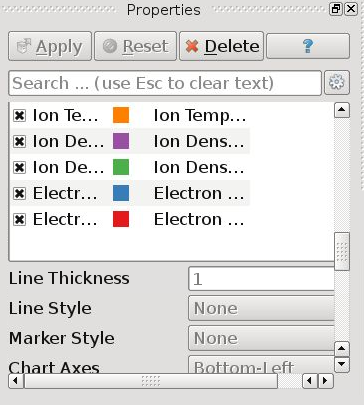
\includegraphics[scale=0.5,trim=0cm 0cm 0cm 0cm,clip]{31_pov4}
    \caption{Data Array scalars selection}
    \label{fig:pv_pov4}
\end{figure}

The axis range settings can be found furthermore in the \textit{Pipeline Browser} as \textbf{Left Axis Range} and \textbf{Bottom Axis Range}.

\begin{figure}[!htb] \centering
    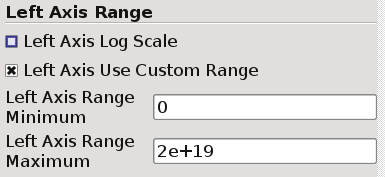
\includegraphics[scale=0.5,trim=0cm 0cm 0cm 0cm,clip]{32_pov5}
    \caption{Axis range customization}
    \label{fig:pv_pov5}
\end{figure}

\clearpage
To crate more Line Charts for the same case click one of the window splitting tools found in the top right corner of the \textit{View Browser} such as \textbf{Split vertical} as seen in Fig. \ref{fig:pv_pov6}. It will open a new separated window and there click \textbf{Line Chart View}, as shown in Fig. \ref{fig:pv_pov7}, and new Line Chart will be created, as seen in Fig. \ref{fig:pv_pov8}. 
\begin{figure}[!htb] \centering
    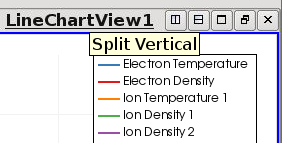
\includegraphics[scale=0.5,trim=0cm 0cm 0cm 0cm,clip]{33_pov6}
    \caption{View Browser Split Vertical}
    \label{fig:pv_pov6}
\end{figure}

\begin{figure}[ht] \centering
\begin{minipage}[b]{0.48\textwidth}
    \centering
    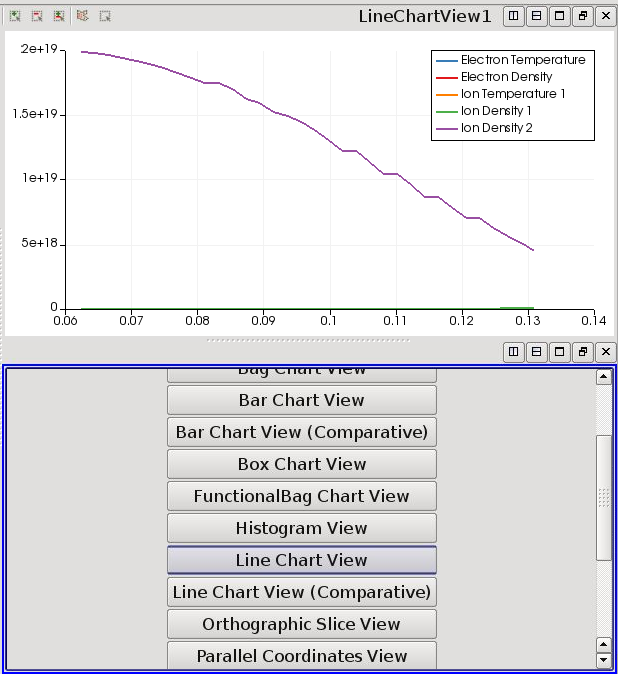
\includegraphics[scale=0.45,trim=0cm 0cm 0cm 0cm,clip]{34_pov7}
    \caption{}
    \label{fig:pv_pov7}
\end{minipage}\hfill
\begin{minipage}[b]{0.48\textwidth}
    \centering
    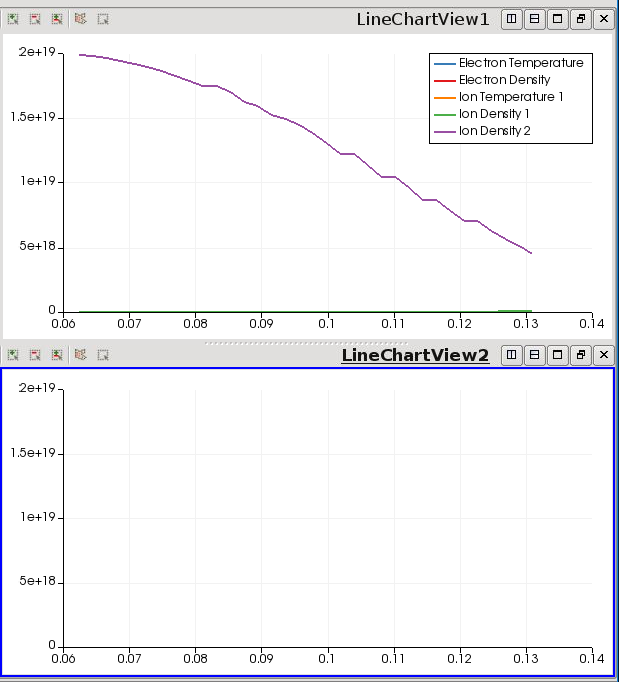
\includegraphics[scale=0.45,trim=0cm 0cm 0.15cm 0cm,clip]{35_pov8}
    \caption{}
    \label{fig:pv_pov8}
\end{minipage}
\end{figure}

\clearpage
Then, while the created empty \textit{Line Chart} is selected\footnote[1]{Notice the blue outline around the View in the \textit{View Browser}}, in the \textit{Pipeline Browser} click on the eye icon beside the \textit{TextOverLine} filter name, which should be transparent by default, as seen in Fig. \ref{fig:pv_pov9}. The by default selected Data Arrays should appear in the \textit{Line Chart}.

\begin{figure}[!htb] \centering
    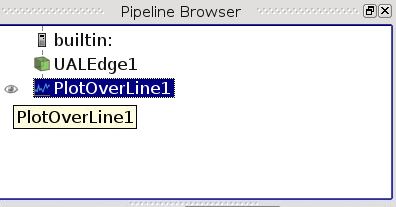
\includegraphics[scale=0.5,trim=0cm 0cm 0cm 0cm,clip]{36_pov9}
    \caption{Hide/Show indicator}
    \label{fig:pv_pov9}
\end{figure}

From there we can work with the chart normally and chose wanted Data Arrays in the \textit{Series Parameters} under \textit{Pipeline Browser} as before. Just note that the \textit{Text Chart} we want to change must first be selected in the \textit{View Browser} before we can operate with it\footnote[2]{The same goes for any View in the \textit{View Browser}}.

An example of using multiple Line Charts is shown in Fig. \ref{fig:pv_pov10}.

\begin{figure}[!htb] \centering
    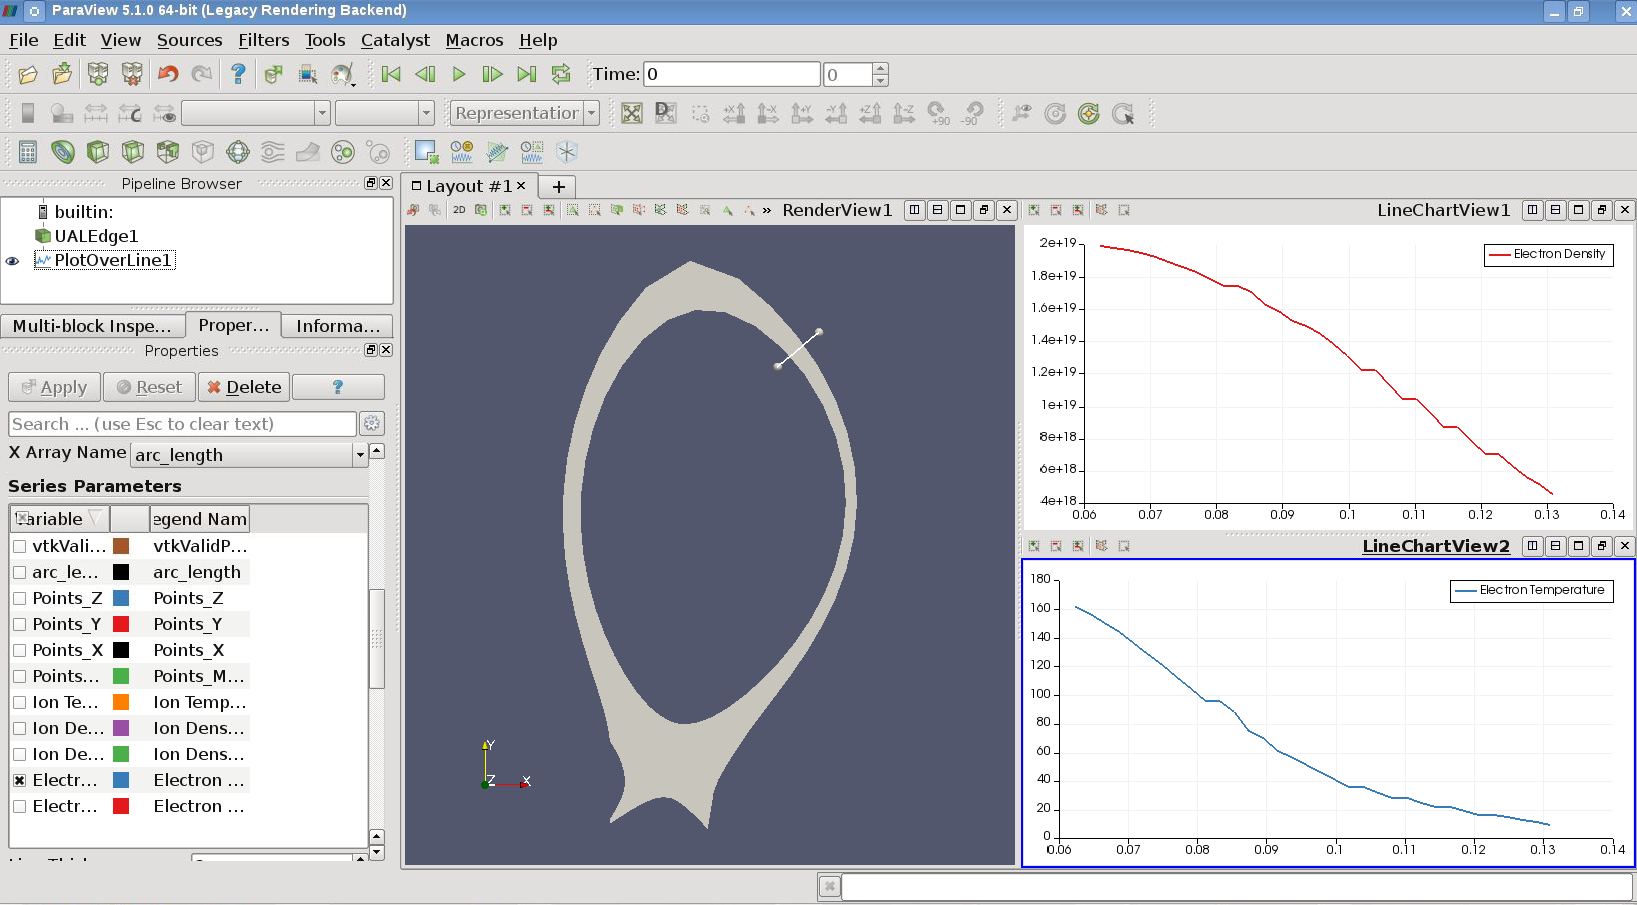
\includegraphics[scale=0.35,trim=0cm 0cm 0cm 0cm,clip]{37_pov10}
    \caption{Example of ordered Line Charts}
    \label{fig:pv_pov10}
\end{figure}




\end{document}

